\documentclass[12pt,a4paper,oneside]{article}
\usepackage[utf8]{inputenc}
\usepackage[english, russian]{babel}
\usepackage[resetfonts]{cmap}

\usepackage{graphicx}
\RequirePackage{float}
\graphicspath{{Drawable/}}
\usepackage[table,xcdraw]{xcolor}

\renewcommand\familydefault{\sfdefault}

\usepackage{tabu}
\usepackage{longtable} %tabu needs this to be loaded.
\usepackage{lipsum} % provides dummy text.

\usepackage{geometry} % Меняем поля страницы.
\geometry{left=2cm} %Левое поле.
\geometry{right=2cm} %Правое поле.
\geometry{top=2cm} %Верхнее поле.
\geometry{bottom=2cm} %Нижнее поле.

\usepackage{amsthm,amssymb,amsmath}

\usepackage{longtable}
\usepackage{color}
\usepackage{xcolor}
\usepackage{listings}
\usepackage{sectsty}
\sectionfont{\Large}

\subsectionfont{\normalsize}
\subsubsectionfont{\small}
 

\usepackage{caption}
\DeclareCaptionFont{white}{\color{white}}
\DeclareCaptionFormat{listing}{\colorbox{gray}{\parbox{\dimexpr\textwidth-1.72\fboxsep\relax}{#1#2#3}}}
\captionsetup[lstlisting]{format=listing,labelfont=white,textfont=white,margin=0pt}
\lstset{language=C,
	numbers=left,
	keepspaces=true,
	tabsize=4,               
	frame=single,                           % Single frame around code
	basicstyle=\small\ttfamily,             % Use small true type font                         
	rulecolor=\color{black},
	captionpos=b,
	showstringspaces=false,	
	abovecaptionskip=-0.9pt,
	xleftmargin=3.4pt,
	xrightmargin=2.6pt,
	breaklines=true,
	postbreak=\raisebox{0ex}[0ex][0ex]{\ensuremath{\color{black}\hookrightarrow\space}},
	xleftmargin=3.2pt,
	escapechar=\&,
	literate={а}{{\selectfont\char224}}1
	{~}{{\textasciitilde}}1
	{б}{{\selectfont\char225}}1
	{в}{{\selectfont\char226}}1
	{г}{{\selectfont\char227}}1
	{д}{{\selectfont\char228}}1
	{е}{{\selectfont\char229}}1
	{ё}{{\"e}}1
	{ж}{{\selectfont\char230}}1
	{з}{{\selectfont\char231}}1
	{и}{{\selectfont\char232}}1
	{й}{{\selectfont\char233}}1
	{к}{{\selectfont\char234}}1
	{л}{{\selectfont\char235}}1
	{м}{{\selectfont\char236}}1
	{н}{{\selectfont\char237}}1
	{о}{{\selectfont\char238}}1
	{п}{{\selectfont\char239}}1
	{р}{{\selectfont\char240}}1
	{с}{{\selectfont\char241}}1
	{т}{{\selectfont\char242}}1
	{у}{{\selectfont\char243}}1
	{ф}{{\selectfont\char244}}1
	{х}{{\selectfont\char245}}1
	{ц}{{\selectfont\char246}}1
	{ч}{{\selectfont\char247}}1
	{ш}{{\selectfont\char248}}1
	{щ}{{\selectfont\char249}}1
	{ъ}{{\selectfont\char250}}1
	{ы}{{\selectfont\char251}}1
	{ь}{{\selectfont\char252}}1
	{э}{{\selectfont\char253}}1
	{ю}{{\selectfont\char254}}1
	{я}{{\selectfont\char255}}1
	{А}{{\selectfont\char192}}1
	{Б}{{\selectfont\char193}}1
	{В}{{\selectfont\char194}}1
	{Г}{{\selectfont\char195}}1
	{Д}{{\selectfont\char196}}1
	{Е}{{\selectfont\char197}}1
	{Ё}{{\"E}}1
	{Ж}{{\selectfont\char198}}1
	{З}{{\selectfont\char199}}1
	{И}{{\selectfont\char200}}1
	{Й}{{\selectfont\char201}}1
	{К}{{\selectfont\char202}}1
	{Л}{{\selectfont\char203}}1
	{М}{{\selectfont\char204}}1
	{Н}{{\selectfont\char205}}1
	{О}{{\selectfont\char206}}1
	{П}{{\selectfont\char207}}1
	{Р}{{\selectfont\char208}}1
	{С}{{\selectfont\char209}}1
	{Т}{{\selectfont\char210}}1
	{У}{{\selectfont\char211}}1
	{Ф}{{\selectfont\char212}}1
	{Х}{{\selectfont\char213}}1
	{Ц}{{\selectfont\char214}}1
	{Ч}{{\selectfont\char215}}1
	{Ш}{{\selectfont\char216}}1
	{Щ}{{\selectfont\char217}}1
	{Ъ}{{\selectfont\char218}}1
	{Ы}{{\selectfont\char219}}1
	{Ь}{{\selectfont\char220}}1
	{Э}{{\selectfont\char221}}1
	{Ю}{{\selectfont\char222}}1
	{Я}{{\selectfont\char223}}1,
	extendedchars=true
}
\newcommand\textbox[1]{%
	\parbox{.5\textwidth}{#1}%
}

\begin{document}
	%%%%%%%%%%%%%%%%%%%%%%%%%%%%%%%%%%%%%%%%%%%%%%%
	%http://i373.spb.ru/file/AndrLectTAU.pdf 40 страница +- 10 страниц
	%%%%%%%%%%%%%%%%%%%%%%%%%%%%%%%%%%%%%%%%%%%%%%%
\noindent\textbox{\textbf{Домашнее задание к лекции 4}\hfill}\textbox{\hfill \textbf{Раскин Д.В. 43501/3}}
\section*{Матрица А канонической формы модели ВСВ}
Передаточная функция задана в следующем виде:

$W(s)=\frac{b_m\prod_{j=1}^{m}(s-s_j)}{a_n\prod_{i=1}^{m}(s-s_i)}=\frac{R(s)}{Q(s)}$

Корни могут иметь различный вид и кратность. Рассмотрим следующие случаи:\\\\
\textbf{Простые вещественные корни}

Пусть $s_i$ - простые, т.е. $s_i\neq s_j$ при $i\neq j$, где $i,j=1,...,n$ и кроме того, они вещественные: $Im s_i=0$. В этом случае матрица А является диагональной матрицей $A=diag\{s_1, s_2,..., s_n\}$.\\\\
\textbf{Простые вещественные и комплексные корни}

Пусть $s_i$ - простые, т.е. $s_i\neq s_j$ при $i\neq j$, где $i,j=1,...,n$ и кроме того, среди корней присутствует комплексно-сопряженные пары корней: $s_{i,i+1}=\alpha_i\pm j\beta_i, j^2=-1$. В этом случае матрица А является квазидиагональной(блочно-диагональной):

\begin{figure}[H]
	\centering
	\begin{minipage}{.4\textwidth}
		\centering
		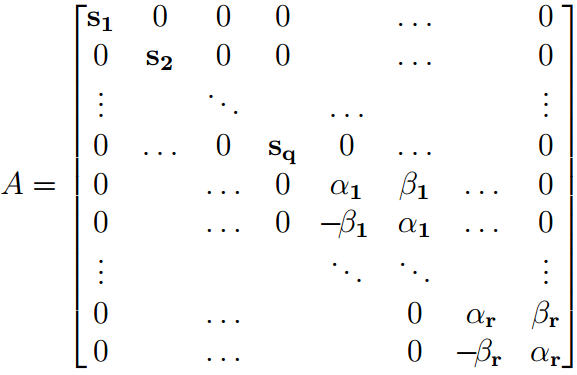
\includegraphics[width=9cm]{Drawable/1}
	\end{minipage}%
	\begin{minipage}{.4\textwidth}
		\centering
		(1)
	\end{minipage}
\end{figure}


Вещественным корням $s_1,s_2,...,s_n$ соответствуют блоки размера 1x1, мнимым корням $s_{q+2i-1,q+2i}=\alpha_i\pm j\beta_i,i=1,2,...,r$ соответствуют блоки размера 2x2 вида:
\begin{figure}[H]
	\centering
	\begin{minipage}{.2\textwidth}
		\centering
		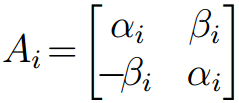
\includegraphics[width=3cm]{Drawable/2}
	\end{minipage}%
	\begin{minipage}{.2\textwidth}
		\centering
		(2)
	\end{minipage}
\end{figure}
\textbf{Кратные вещественные и комплексные корни}

Пусть имеется кратные корни: $s_1$ - кратности $l_1,s_2$ - кратности $l_2,...,s_p$ - кратности $l_p$. Выполнено условие $\sum_{i=1}^{p}l_i=n$. Тогда матрица А имеет следующую блочную структуру:

\begin{figure}[H]
	\centering
	\begin{minipage}{.25\textwidth}
		\centering
		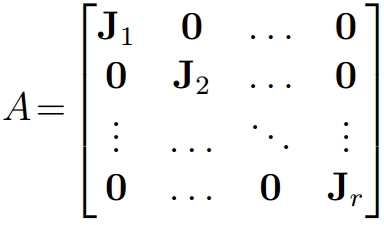
\includegraphics[width=4.5cm]{Drawable/3}
	\end{minipage}%
	\begin{minipage}{.25\textwidth}
		\centering
		(3)
	\end{minipage}
\end{figure}
где $J_i, i=1,2,...,r,$ r - клетки(ящики) Жордана, имеющие вид: 

-- для вещественных корней($Ims_j=0$)
\begin{figure}[H]
	\centering
	\begin{minipage}{.4\textwidth}
		\centering
		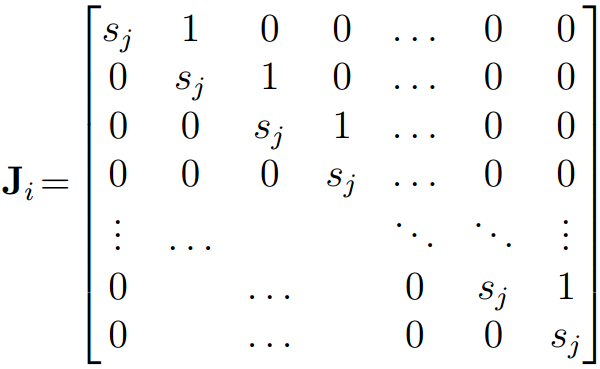
\includegraphics[width=9cm]{Drawable/4}
	\end{minipage}%
	\begin{minipage}{.4\textwidth}
		\centering
		(4)
	\end{minipage}
\end{figure}
-- для мнимых собственных чисел $s_j=\alpha_j\pm j\beta_j$
\begin{figure}[H]
	\centering
	\begin{minipage}{.5\textwidth}
		\centering
		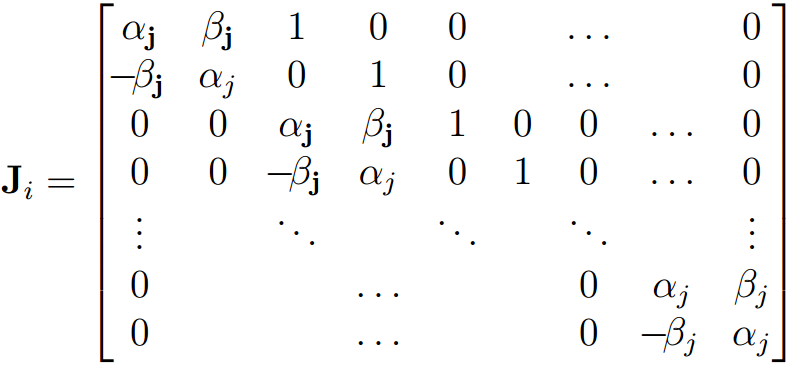
\includegraphics[width=11cm]{Drawable/5}
	\end{minipage}%
	\begin{minipage}{.5\textwidth}
		\centering
		(5)
	\end{minipage}
\end{figure}
Блочно-диагональная форма матрицы А вида (3) называется вещественной(обобщенной) жордановой матрицей.

Размер каждой клетки J вида (4) может быть от 1х1 до $l_j$х$l_j$, а размеры клеток $J_i$ вида (5) -- от 2х2 до $2l_j$х$2l_j$ (где j - кратность корня $s_j$). Следовательно, в случае простых корней клетки, отвечающие вещественным корня, имеют порядок один: $J_i=s_i$, а клетки, отвечающие комплексным корням - порядок два: $J_i= \begin{bmatrix} \alpha_i & \beta_i  \\ -\beta_i & \alpha_i \end{bmatrix}$. Таким образом, форма (1) следует из (3) как частный случай.

\section*{Эквивалентные преобразования форм модели ВСВ}
Обратимся теперь к задаче перехода от исходных уравнений состояния к уравнениям в заданной канонической форме. Решение этой задачи сводится к определению невырожденной n x-матрицы T такой, что для заданных матриц A, B, C получаются уравнения с матрицами $\widetilde{A}=TAT^{-1}, \widetilde{B}=TB, \widetilde{C}=CT^{-1}$, имеющими требуемый канонический вид.\\\\
\textbf{1. Преобразование к канонической форме}

\textbf{Простые вещественные корни}

Если все корни характеристического многочлена матрицы А - простые вещественные числа, тогда матрица приведения Т к диагональной канонической форме (1) определяется из выражения:
\begin{center}
$T=[x^0_1, x^0_2,..., x^0_n]^{-1}$
\end{center}
где $x^0_i(i=1,2,...,n)$ - собственные векторы матрицы А.\\\\
\textbf{Простые вещественные и комплексные корни}

Если размер каждой клетки совпадает с кратностью соответствующего вещественного собственного значения или равен удвоенной кратности мнимых
(комплексно-сопряженных) собственных значений, то такая матрица может быть приведена к виду Фробениуса. В противном случае такая возможность отсутствует.

Рассматривая алгоритмы приведения уравнений состояния к формам НФУ и НФН, будем считать, что преобразование матрицы А к виду Фробениуса возможно.\\\\
\textbf{2. Управляемое каноническое представление}

Введем nxn-матрицы(управляемости)
\begin{center}
$Q=[b, Ab, ..., A^{n-1}b], \widetilde{Q}=[\widetilde{b}, \widetilde{Ab}, ..., \widetilde{A}^{n-1}\widetilde{b}]$
\end{center}
Если выполнены условия:
\begin{center}
$det(sI_n-A)\equiv det(sI_n-\widetilde{A}, detQ\neq0, det\widetilde{Q}\neq0)$, 
\end{center}
то существует и единственна невырожденная матрица преобразования Т, определяемая выражением
\begin{center}
	$T=\widetilde{Q}Q^{-1}$
\end{center}
при которой матрицы A,b и $\widetilde{A}, \widetilde{b}$ связаны соотношением:
\begin{center}
	$\widetilde{A}=TAT^{-1}, \widetilde{b}=Tb$
\end{center}
\textbf{3. Наблюдаемое каноническое представление}

Введем nxn-матрицы(наблюдаемости)
\begin{center}
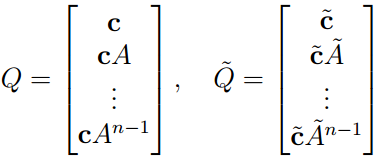
\includegraphics[width=5cm]{Drawable/6}
\end{center}
При выполнении условий
\begin{center}
$det(sI_n-A)\equiv det(sI_n-\widetilde{A}, detQ\neq 0, det\widetilde{Q}\neq0$
\end{center}
существует и единственна невырожденная матрица преобразования
\begin{center}
	$T=\widetilde{Q}^{-1}Q$
\end{center}
так что матрицы A, с и $\widetilde{A}, \widetilde{c}$ связаны соотношением
\begin{center}
 $\widetilde{A}=TAT^{-1}, \widetilde{c}=cT^{-1}$
\end{center}

%%%%%%%%%%%%%%%%%%%%%%%%%%%%%%%%%%%%%%%%%%%%%%%
% тут не точно
%%%%%%%%%%%%%%%%%%%%%%%%%%%%%%%%%%%%%%%%%%%%%%%
Всегда есть множитель $\lambda\in R, \lambda\neq0$ такой, что $x^0_i, \lambda x^0_{i+1}$ - комплексно-сопряженные. Поэтому будем считать, что выполнено условие $x^0_{i+1}=conj(x^0_i)$, где conj - операция комплексного сопряжения. Определим теперь векторы $h_i, h_{i+1}$ формулами
\begin{center}
$h_i=\frac{1}{2}(x^0_i+x^0_{i+1}), h_{i+1}=\frac{1}{2\jmath}(x^0_i+x^0_{i+1})$
\end{center}
Векторы $h_i, h_{i+1}$ по построению вещественные и, если все собственные числа простые, линейно независимы между собой и с другими собственными векторами. Эти векторы определяют в пространстве $R^n$ некоторую собственную плоскость – инвариантное подпространство матрицы A размерности два.

Построим теперь матрицу преобразования
\begin{center}
$T=[X^0_1, X^0_2, ..., h_j, h_{j+1}, ..., h_{q+r-1}, h_{q+r}]^{-1}$
\end{center}
где вектор-столбцы $x^0_i$ отвечают вещественным, а $h_j, h_{j+1}$ - мнимым собственным значениям $s_{j,j+1}=\alpha_j\pm\jmath\beta_j$.

Преобразование $\widetilde{A}=TAT^{-1}$ с найденной таким образом матрицей T приводит уравнения системы к вещественной блочно-диагональной форме (1), в которой порядок следования блоков соответствует порядку расположения столбцов $x^0_i, h_j$ у матрицы $P=T^{-1}$.\\\\
\textbf{Кратные вещественные и комплексные корни}\\
Из выражения $\widetilde{A}=TAT^{-1}$, следует что:
\begin{center}
	$\widetilde{A}T=TA$
\end{center}
Обозначим столбцы матрицы Т как $q_1, q_2, ..., q_n$. Тогда из формы (3) матрицы А с учетом предыдущей формулы получим:
\begin{figure}[H]
	\centering
	\begin{minipage}{.2\textwidth}
		\centering
		$Aq_i-\lambda q_i+\gamma_iq{i-1}$
	\end{minipage}%
	\begin{minipage}{.2\textwidth}
		\centering
		(*)
	\end{minipage}
\end{figure}
где $\gamma_i$ принимает значение 0 или 1 в зависимости от А, а $\lambda$ - характеристическое число матрицы А.

Пусть разбиение блока $T_i$ матрицы T, соответствующее разбиению блока $J_i$ - в форме (4) или (5) в зависимости от вида корня - имеет вид $T_{i1}, T_{i2}, ..., T_{il_i}$. Тогда число $\gamma_i$ равно нулю, когда соответствующий столбец $q_i$ матрицы Т является первым столбцом подблока. Так как, при $\gamma_i$ вектор $q_i$ является собственным вектором матрицы А, можно найти первые столбцы каждого подблока как собственные векторы матрицы А. Оставшиеся столбцы каждого подблока тогда получаются из (*) при $\gamma_i=1$. Такие оставшиеся столбцы известны как обобщенные собственные векторы. Этот процесс останавливается, когда (*) обеспечивает получение решения.












\end{document}